\documentclass[preprint,10pt]{elsarticle}

\usepackage{amssymb}
\usepackage{amsmath}
\usepackage{lineno}
\usepackage{hyperref}

\usepackage{epstopdf}
\usepackage{epsfig}
\usepackage{setspace}

\newcommand{\be}{\begin{equation}}
\newcommand{\ee}{\end{equation}}
\newcommand{\beq}{\begin{eqnarray}}
\newcommand{\eeq}{\end{eqnarray}}
\newcommand{\ba}{\begin{eqnarray}}
\newcommand{\ea}{\end{eqnarray}}

\newcommand{\ua}{{\bf u}_\alpha}
\newcommand{\utwo}{\overline{\bf u}_2}
\setcounter{MaxMatrixCols}{24}

\journal{Coastal Engineering}

\begin{document}


%\title{Model derivations}

\begin{center}
{\bf \Large Nesting FUNWAVE in a large-scale wave-averaged model}
 \end{center}
 
 \section{The nesting idea }
 
 \noindent
 Nesting FUNWAVE in a large-scale wave-averaged model has three steps:
 
 \vspace{0.5cm}
 \noindent
 1) interpolate the results, $(u,v,\eta)$, from the large-scale model into the FUNWAVE grid. 
 
 As shown in Figure \ref{two_grid}, the region for the large-scale model output(grid point, red dots ) should cover the entire FUNWAVE grid, avoiding any extrapolation. The grid of the large-scale model should be a structured grid, either curvilinear or rectangular grid. Values at $A$ are obtained from interpolations conducted within the angle (1,2,3) marked in the Figure (see detailed in the next section).  ({\bf Let me know if you prefer JONSWAP, TMA, or data-based spectra. The advantage of using the formula-based spectra (JON or TMA) is that spectral components can be split using an equal-energy method. The wavemaker only needs Hsig, peak period and spreading parameters, which can be obtained from SWAN or WWIII. So you wouldn't worry about how to pre-processing the spectral data.})
 
  \vspace{0.5cm}
 \noindent
 2) incorporate the large-scale model results into long-wave passing sponge layers
 
 Figure \ref{sponge} shows sponge layers as an example. The sponge layers can be configured in any of the four boundaries. In the current case, WEST, SOUTH, and NORTH sponges are specified. The east boundary is the coast. The sponge layers are long-wave passing, meaning the results from the large-scale model can pass through the sponge layers, while absorbing short waves from the inside domain. 
 
  \vspace{0.5cm}
 \noindent
 3) make waves at the wavemaker location
 
 An internal wavemaker should be used for this application. The west boundary wavemaker CANNOT be used due to the application of the WEST sponge. 
 
  \begin{figure}
\begin{center}
 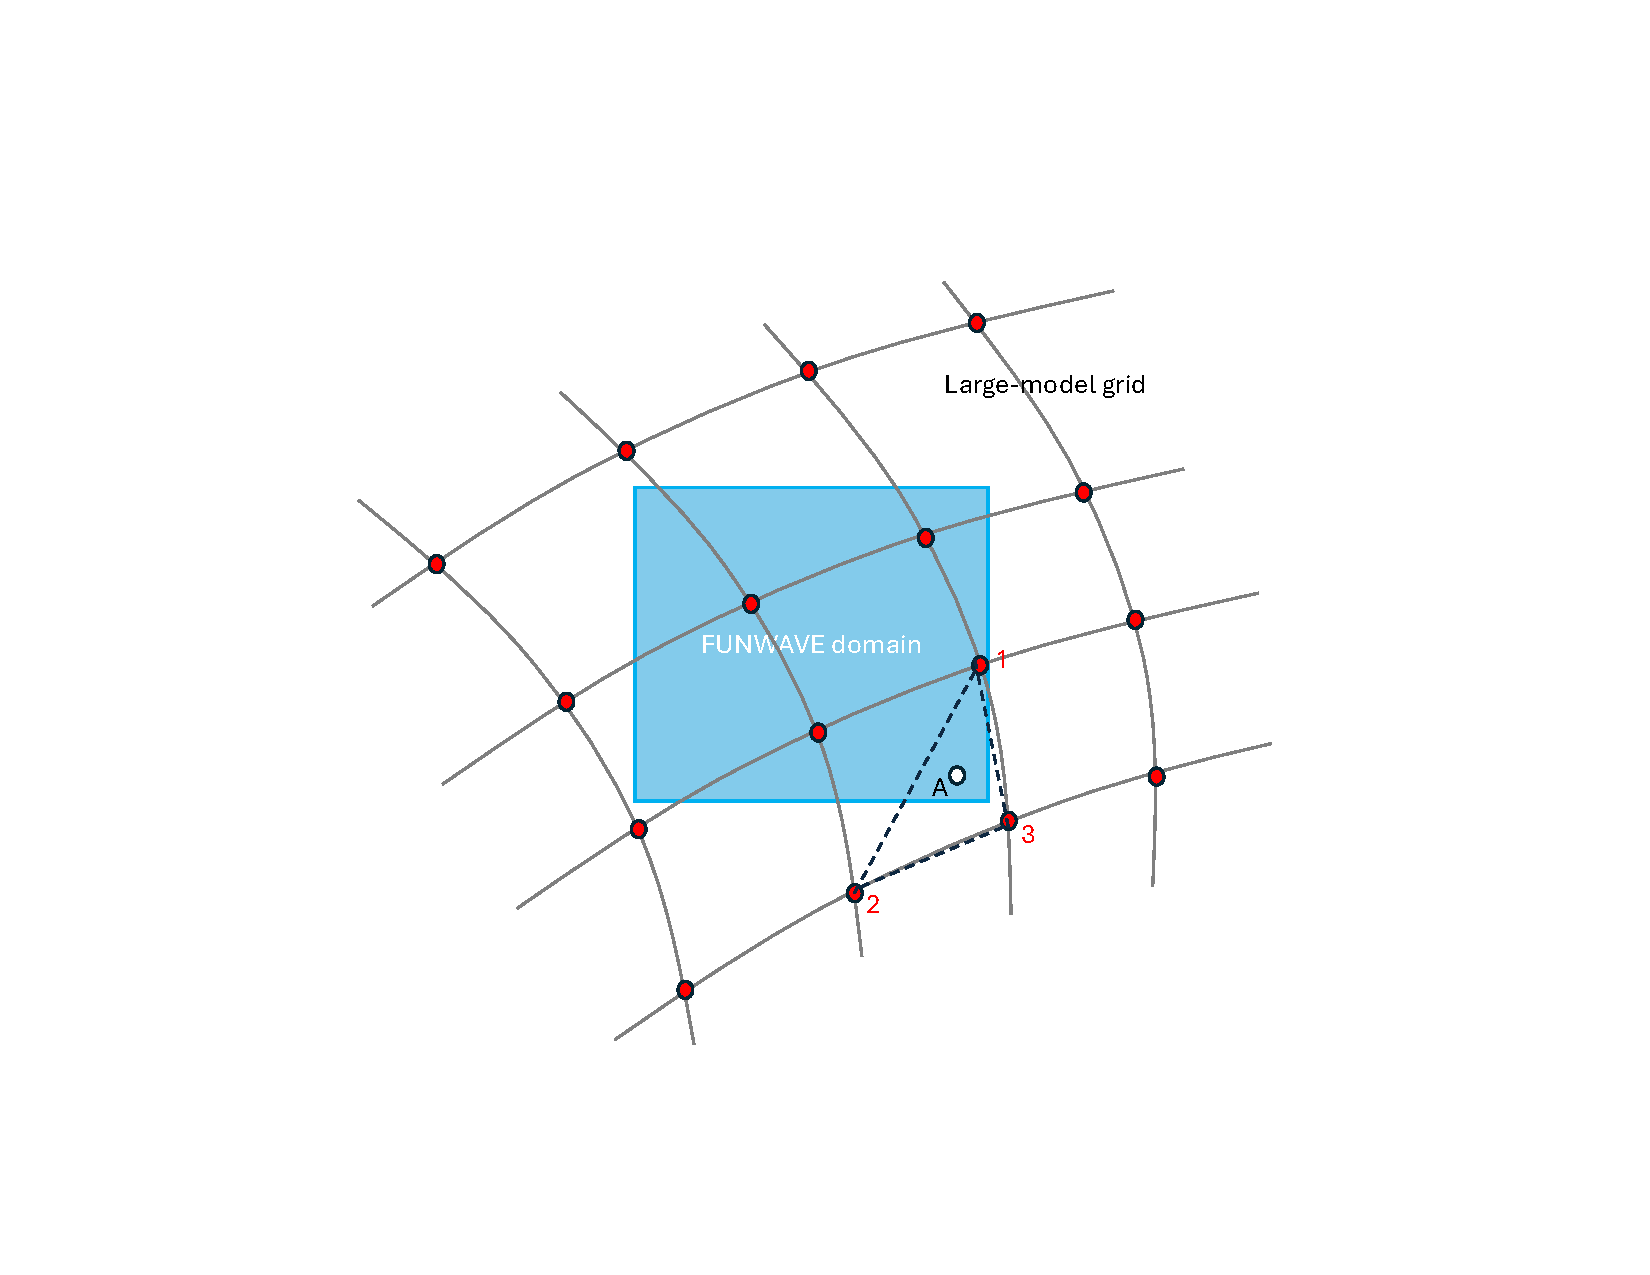
\includegraphics[width=1.0\textwidth]{figures/two_grids.pdf}
 \caption{Interpolation triangle. The dashed triangle is used for the linear interpolation as explained by Figure \ref{triangle} }
 \label{two_grid}
 \end{center}
 \end{figure}
 
  \begin{figure}
\begin{center}
 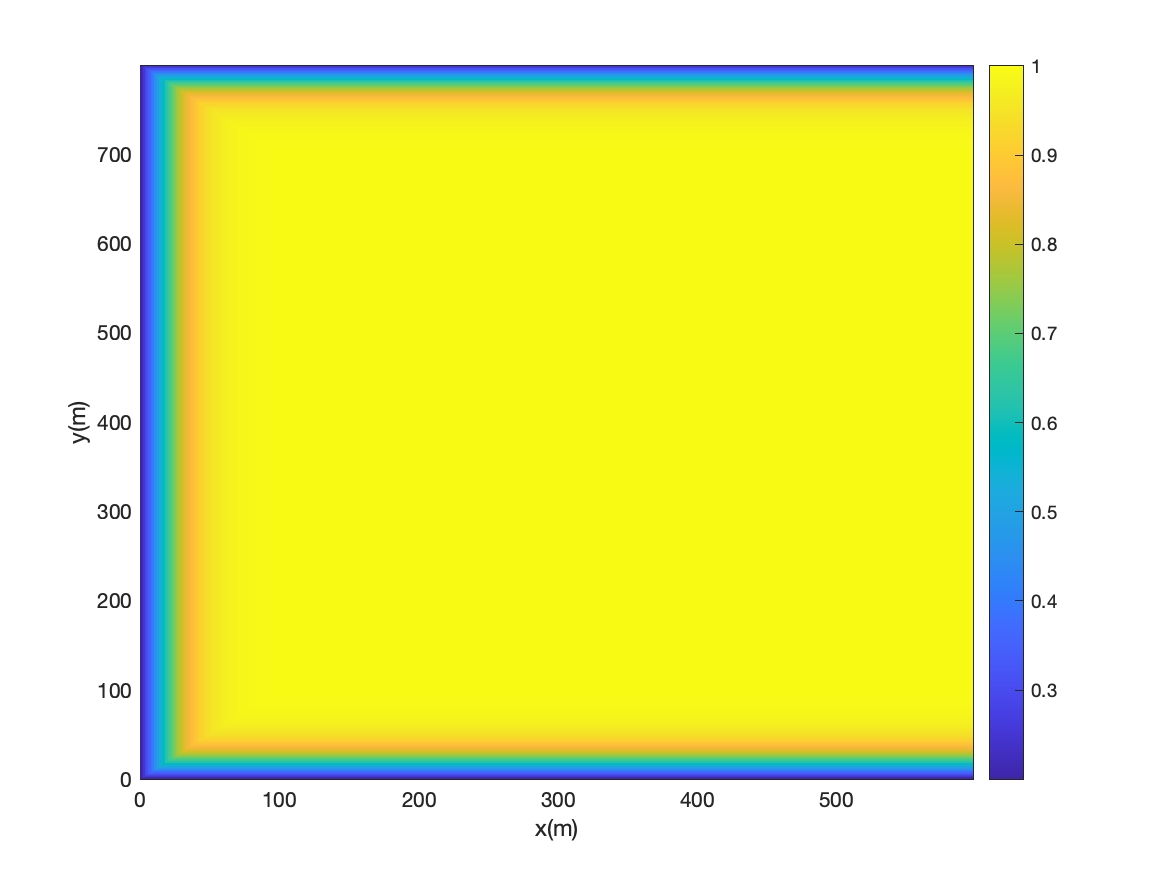
\includegraphics[width=1.0\textwidth]{figures/sponge_2d.jpg}
 \caption{2D sponge layers. In this application, the long-wave passing sponge layers are applied at the west, south, and north boundaries. The east boundary is shoreline. }
 \label{sponge}
 \end{center}
 \end{figure}
 
 \section{Interpolation} 
  
  Interpolation or extrapolation (not suggested) is  employed between a structured grid of a large-scale model
 and a FUNWAVE grid.  A linear interpolation method is performed.
As shown in Figure \ref{triangle}, an interpolation
value at  point $A$ in the FUNWAVE grid is evaluated by the values at three points, $1,
2$ and $3$, of a triangle in the large-scale model grid which surrounds point $A$.  Four triangle areas
$S_{\alpha \beta \gamma}$, i.e., $S_{123}, S_{12A}, S_{31A}$ and $S_{23A}$ are
calculated using the following formula:
  
\ba
S_{\alpha \beta \gamma}=\left | \begin{array}{ccc}x_\alpha & y_\alpha & 1 \\
x_\beta & y_\beta & 1 \\
x_\gamma & y_\gamma &1 
\end{array}
\right |
\ea
where $(x_{\alpha}, y_{\alpha}$) represents
coordinates of point $1, 2, 3$ and $A$.  For interpolation, ($\alpha, \beta,
\gamma$) are  counter-clockwise for all the four triangles and thus $S_{\alpha
\beta \gamma}$ are positive. For extrapolation, clockwise ($\alpha, \beta,
\gamma$) results in negative $S_{\alpha
\beta \gamma}$. The following formula is used for both interpolation and
extrapolation:
\be
F_A=(F_1S_{23A}+F_2 S_{31A} + F_3 S_{12A})/S_{123}
\ee
where $F_1, F_2, F_3$ and $F_A$ represent any converted variables at
point $1, 2, 3 $ and $A$, respectively.

To save computational time for interpolation/extrapolation, $S_{\alpha
\beta \gamma}$ values are stored in the initialization stage (only calculated once).  
  
 \begin{figure}
\begin{center}
 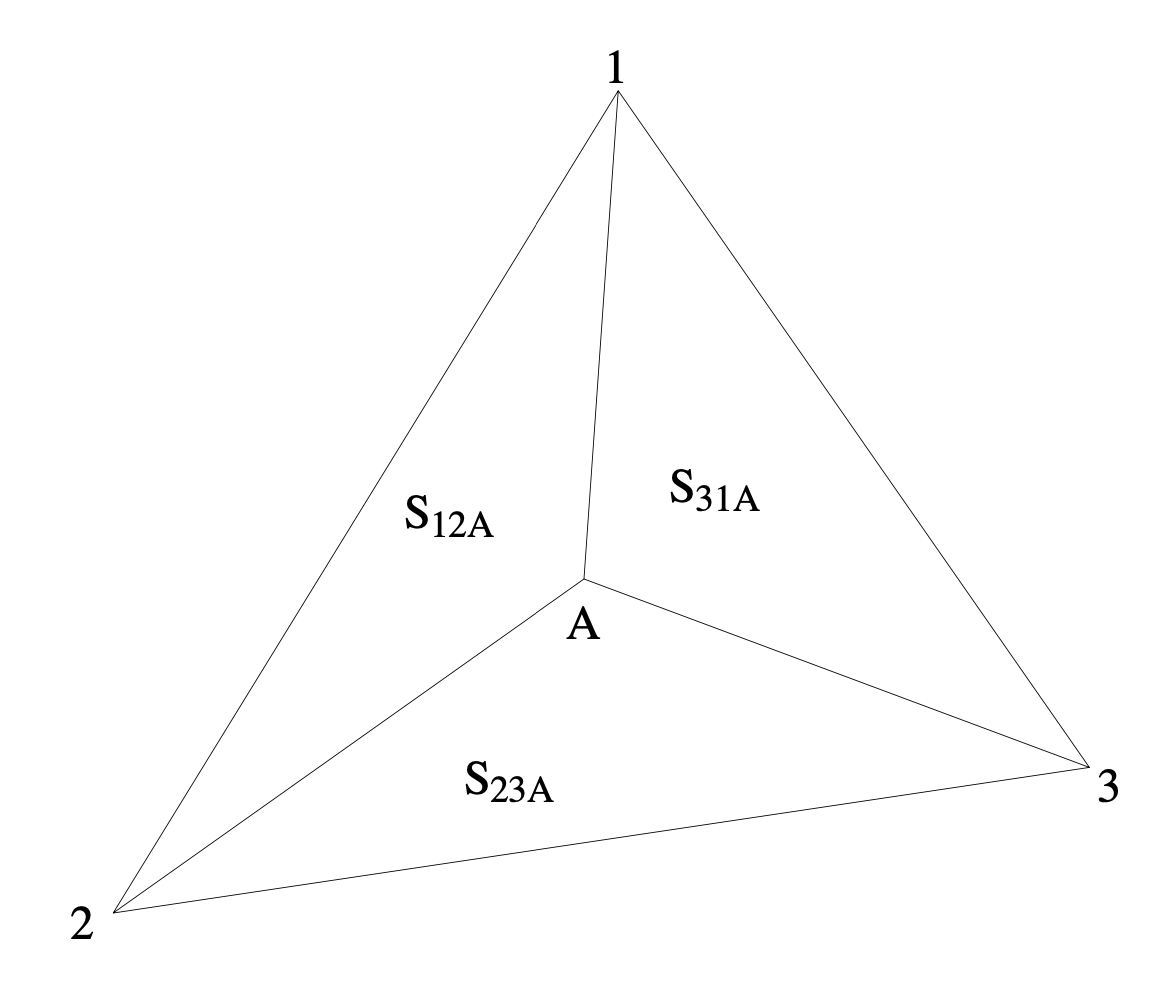
\includegraphics[width=1.0\textwidth]{figures/triangle.png}
 \caption{Interpolation triangle }
 \label{triangle}
 \end{center}
 \end{figure}
  

\section{The new module, 2D nesting module}
   
 The new module is called  `ABS\_GEN\_2D\_MODULE' in mod\_2d\_abs\_gen.F. To activate this module, you should specify 
 
  -DMAP2D\_ABS\_GEN
  
  in Makefile when compiling the the code. In input.txt, the following parameters are needed, for example
  
 \noindent 
MAP2D\_GEN\_ABS = T \\
BC\_WEST\_NEST = T \\
BC\_EAST\_NEST = F \\
BC\_SOUTH\_NEST = T  \\
BC\_NORTH\_NEST = T  \\
MappingDataFileName = large\_model\_data.txt   
 
In this application,  BC\_EAST\_NEST = F is applied, meaning no sponge at the east boundary.  The large-scale model results at the east boundary will not be applied, even they are provided. The long-wave passing boundary conditions will be applied on WEST, SOUTN, and NORTH boundaries only. 

The file, large\_model\_data.txt, contains large-scale model results in time. The following is an example of the data format:

\vspace{0.5cm}
\noindent
eta, u, v data from a large-scale model (void line) \\
2 2 ! M\_DATA N\_DATA (the data grid is 2x2) \\
! 2d x-coordinate (void line) \\
0 1000  (x-coordinates)\\
0 1000  (x-coordinates)\\
! 2d y-coordinate (void line)\\
0 0  (y-coordinates)\\
1200 1200 (y-coordinates) \\
0.0   -time (in second) \\
0.0 0.0 - eta \\
0.0 0.0 \\
0.0 0.0  - u \\
0.0 0.0 \\
0.0  0.0 - v \\
0.0 0.0  \\
500.0   -time \\
0.5 0.1 - eta \\
0.0 0.0 \\
0.0 0.0  - u \\
0.0 0.0 \\
0.0 0.0 - v \\
0.0 0.0  

\section{Long-wave passing sponge and parameters}

The low-passing sponge is based on Larsen and Dancy (1983). Inside the sponge layer, the dependent variables $(\eta, u, v)$ are attenuated 

The damping formula can be expressed as
\be
C_s = -\alpha_s^{\gamma^{i-1}}
\ee
where $i = 1, 2, ... n$. The width of sponge is $(n-1)*dx$.  Figures \ref{R} - \ref{width} show the distributions of the damping coefficient with different $\gamma$,  $\alpha_s$, and width (number of grid points). We choose the default values as   $\gamma$ = 0.85, $\alpha_s$ = 100, and width = 30 points. To change the parameters, you can specify $\gamma$ and  $\alpha_s$ as

R\_sp = float number ($\gamma$)

A\_sp = float number ($\alpha_s$)

\noindent
(We keep the symbols, R\_sp and A\_sp, keeping consistent with the traditional sponge layers. )

To check the sponge layer distribution, use SpongeMap.txt saved in your result folder. You can also check the large-scale model results (interpolated in the FUNWAVE domain). In input.txt, set 

MAP2D\_ETA = T

MAP2D\_U = T

MAP2D\_V = T

You will get output of ($\eta, u, v$) in files eta\_map\_xxxxx, u\_map\_xxxxx, and v\_map\_xxxxx. 

 \begin{figure}
\begin{center}
 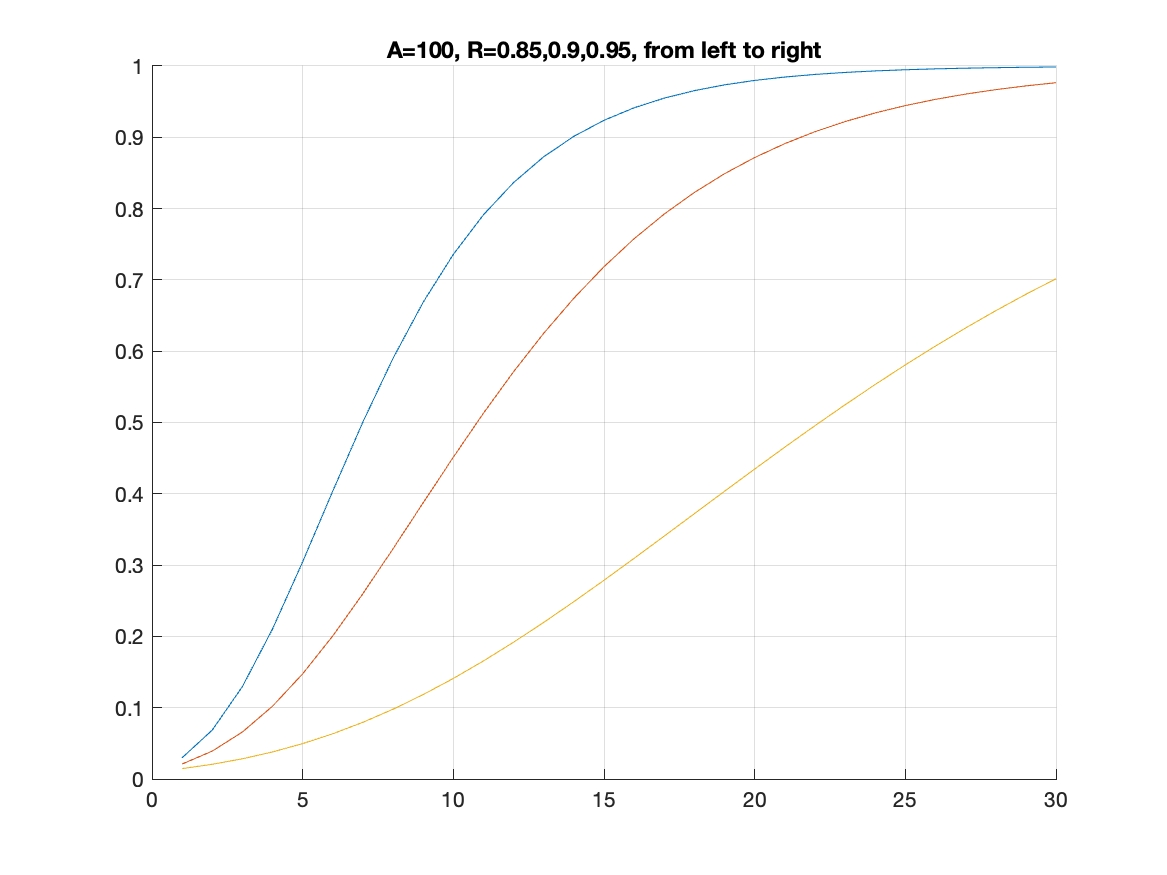
\includegraphics[width=0.8\textwidth]{figures/test_sponge_R.jpg}
 \caption{Distribution of damping coefficient with different $\gamma$ (R in code) }
 \label{R}
 \end{center}
 \end{figure}  

 \begin{figure}
\begin{center}
 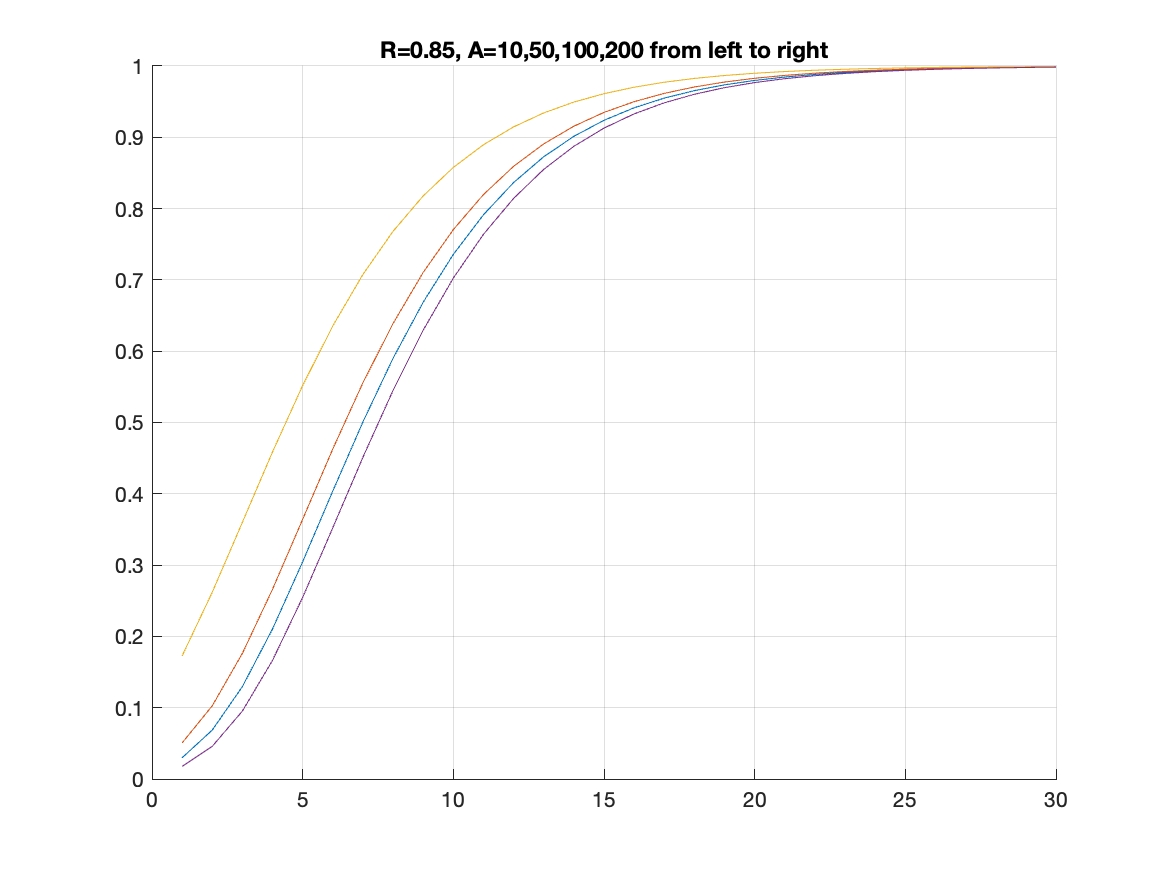
\includegraphics[width=0.8\textwidth]{figures/test_sponge_A.jpg}
 \caption{Distribution of damping coefficient with different $\alpha_s$ (A in code) }
 \label{A}
 \end{center}
 \end{figure}  
 
  \begin{figure}
\begin{center}
 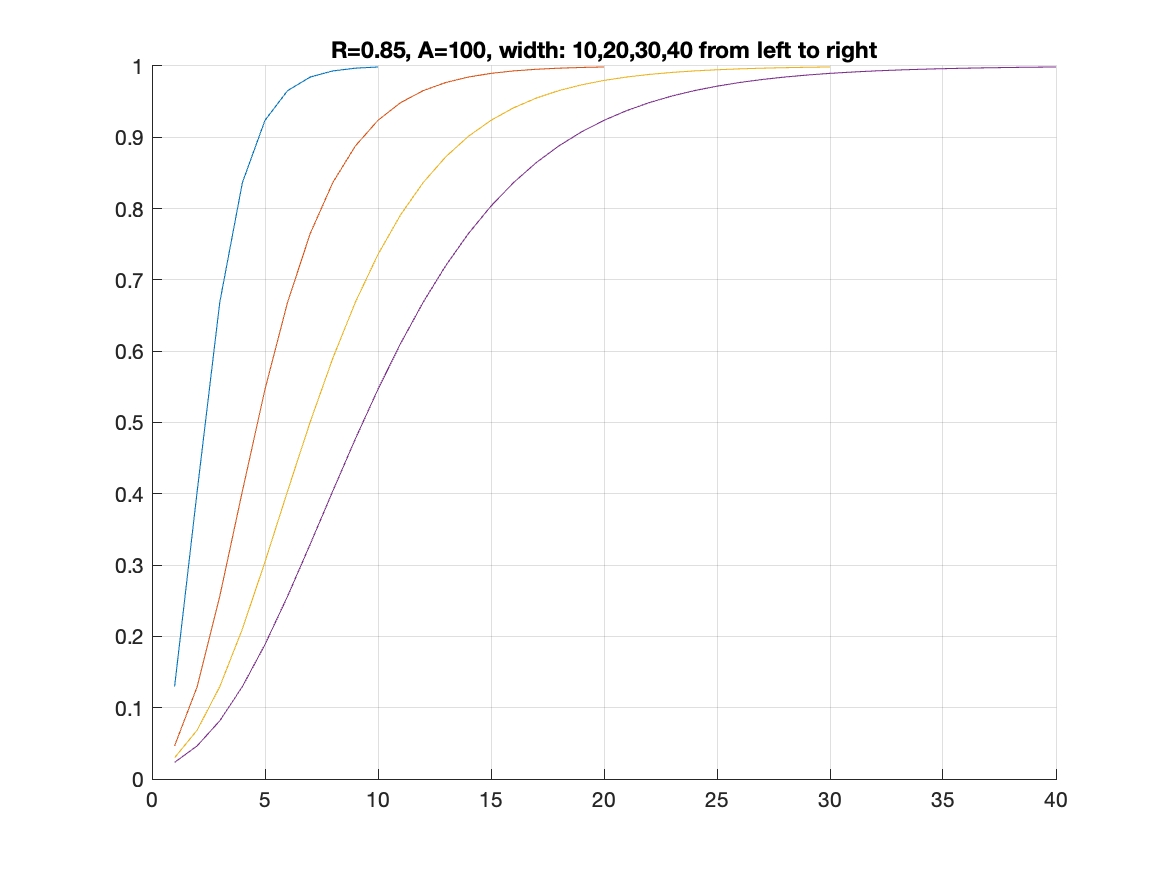
\includegraphics[width=0.8\textwidth]{figures/test_sponge_width.jpg}
 \caption{Distribution of damping coefficient with different width of sponge layer (number of grid points) }
 \label{width}
 \end{center}
 \end{figure}  
   
\section{Example and results}

The example can be found in /nest\_large\_model/. Procedures:

1) compile the code in the example folder

2) check input.txt, given in the example folder

3) run the model

4) matlab scripts can be found in /postprocessing/

\vspace{0.5cm}
\noindent
In this example,  the large-scale model results are specified in large\_model\_data.txt, as shown in the last section. Four grid points (2x2) in the large-scale model  are used, with x-coordinate range of (0 1000) and y-coordinate range of (0 1200) in meters. Note that the reference is (0,0), which is the origin of the FUNWAVE coordinates. A surface slope (eta) is specified, changing with time from 0 to 500 s. Zero velocity is specified on purpose of surface gradient driven currents. 

Figure \ref{surface} shows the surface elevation at 399 s, with the FUNWAVE result on the left, and the large-model result on the right. The large-scale slope can be seen in the FUNWAVE result, indicating the large-scale model results pass through the sponge layers. The slope can also be shown in the wave-averaged elevation from FUNWAVE (Figure \ref{mean}, left), in comparison with the large-scale data (right). 

 \begin{figure}
\begin{center}
 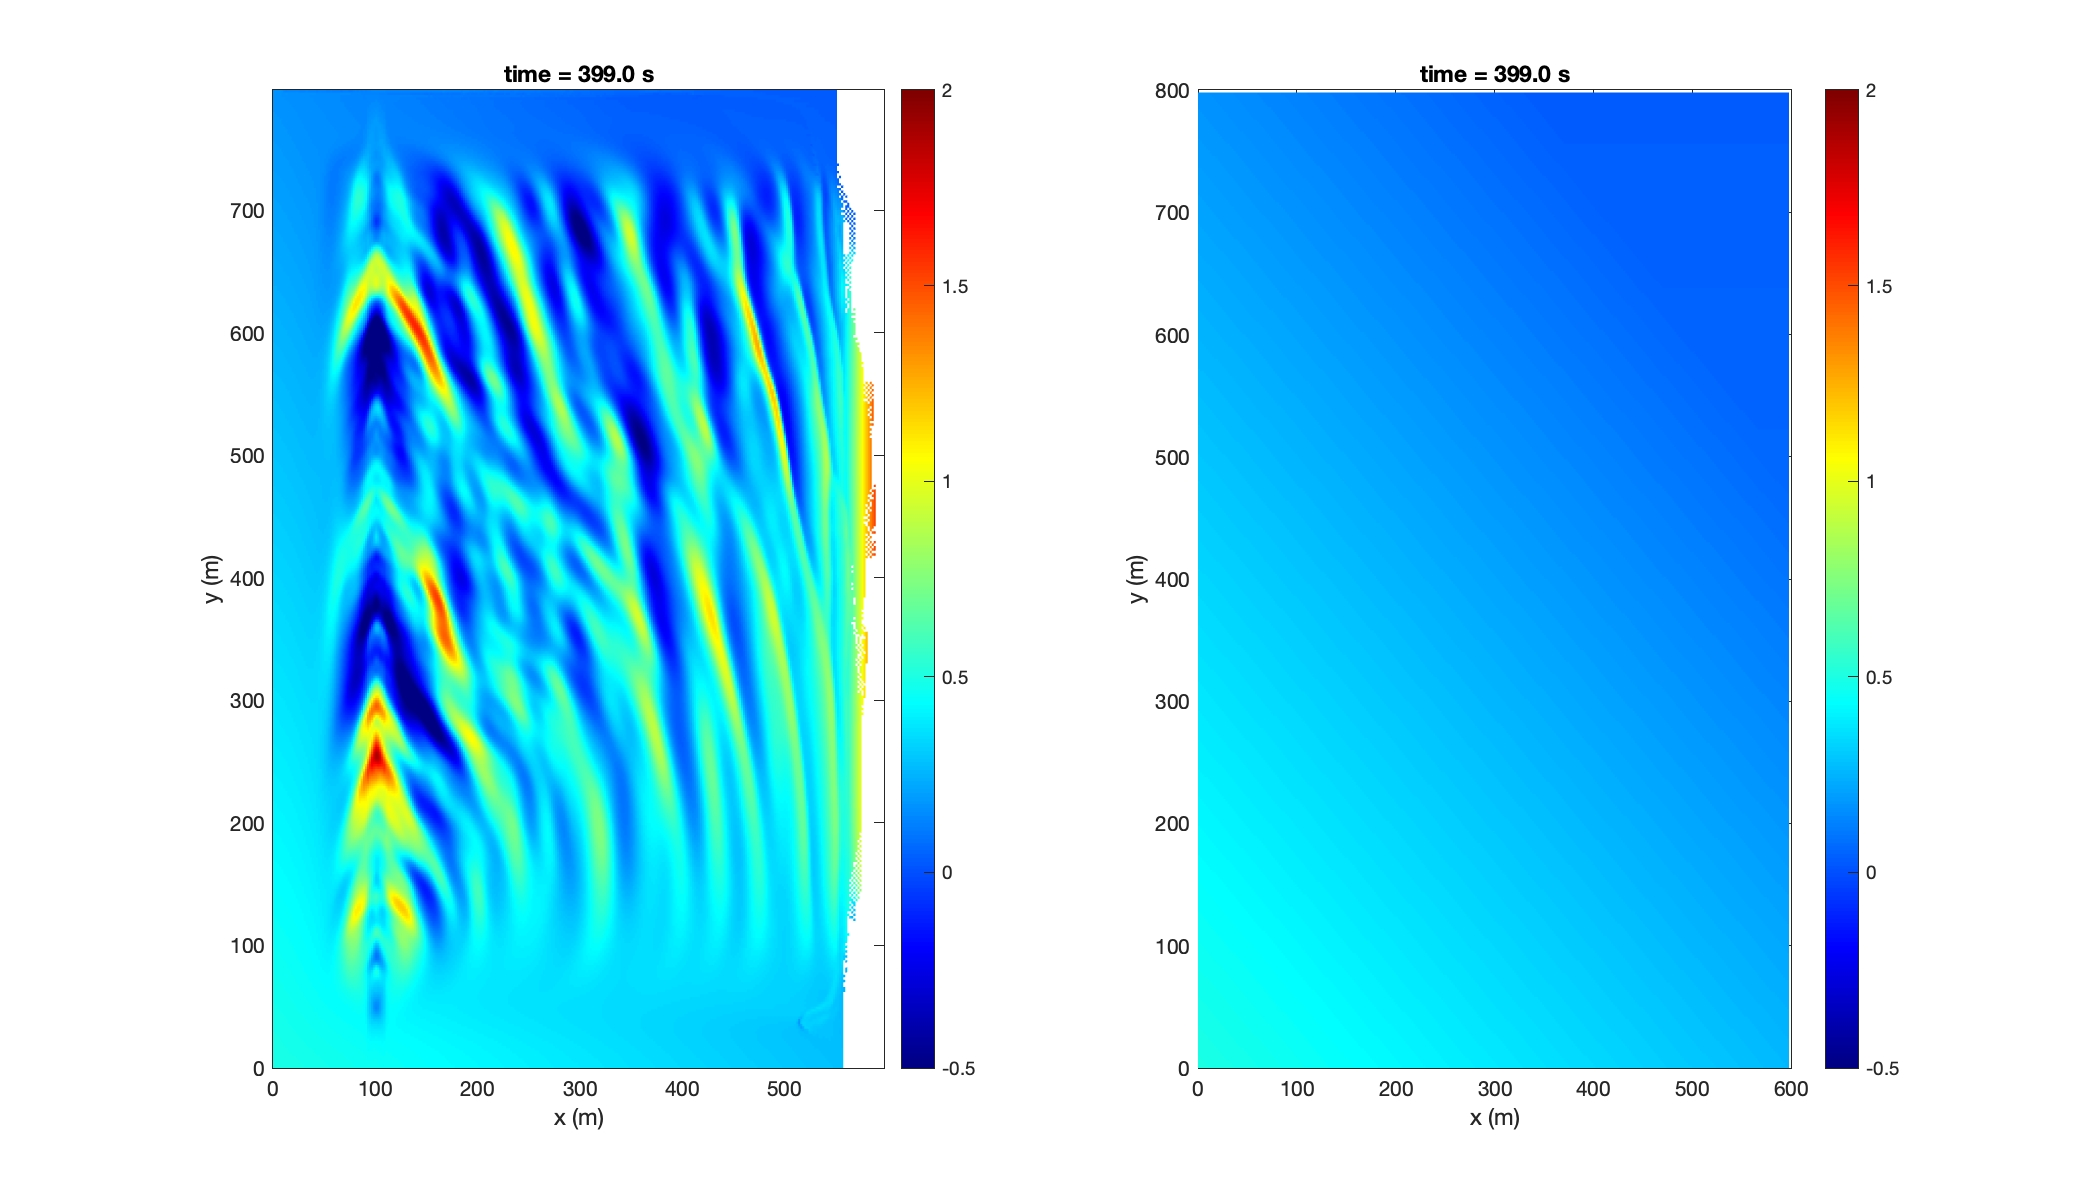
\includegraphics[width=1.0\textwidth]{figures/elevation_view.jpg}
 \caption{Left: surface elevation from FUNWAVE; right: surface elevation interpolated from the large-scale model }
 \label{surface}
 \end{center}
 \end{figure}  
  
  \begin{figure}
\begin{center}
 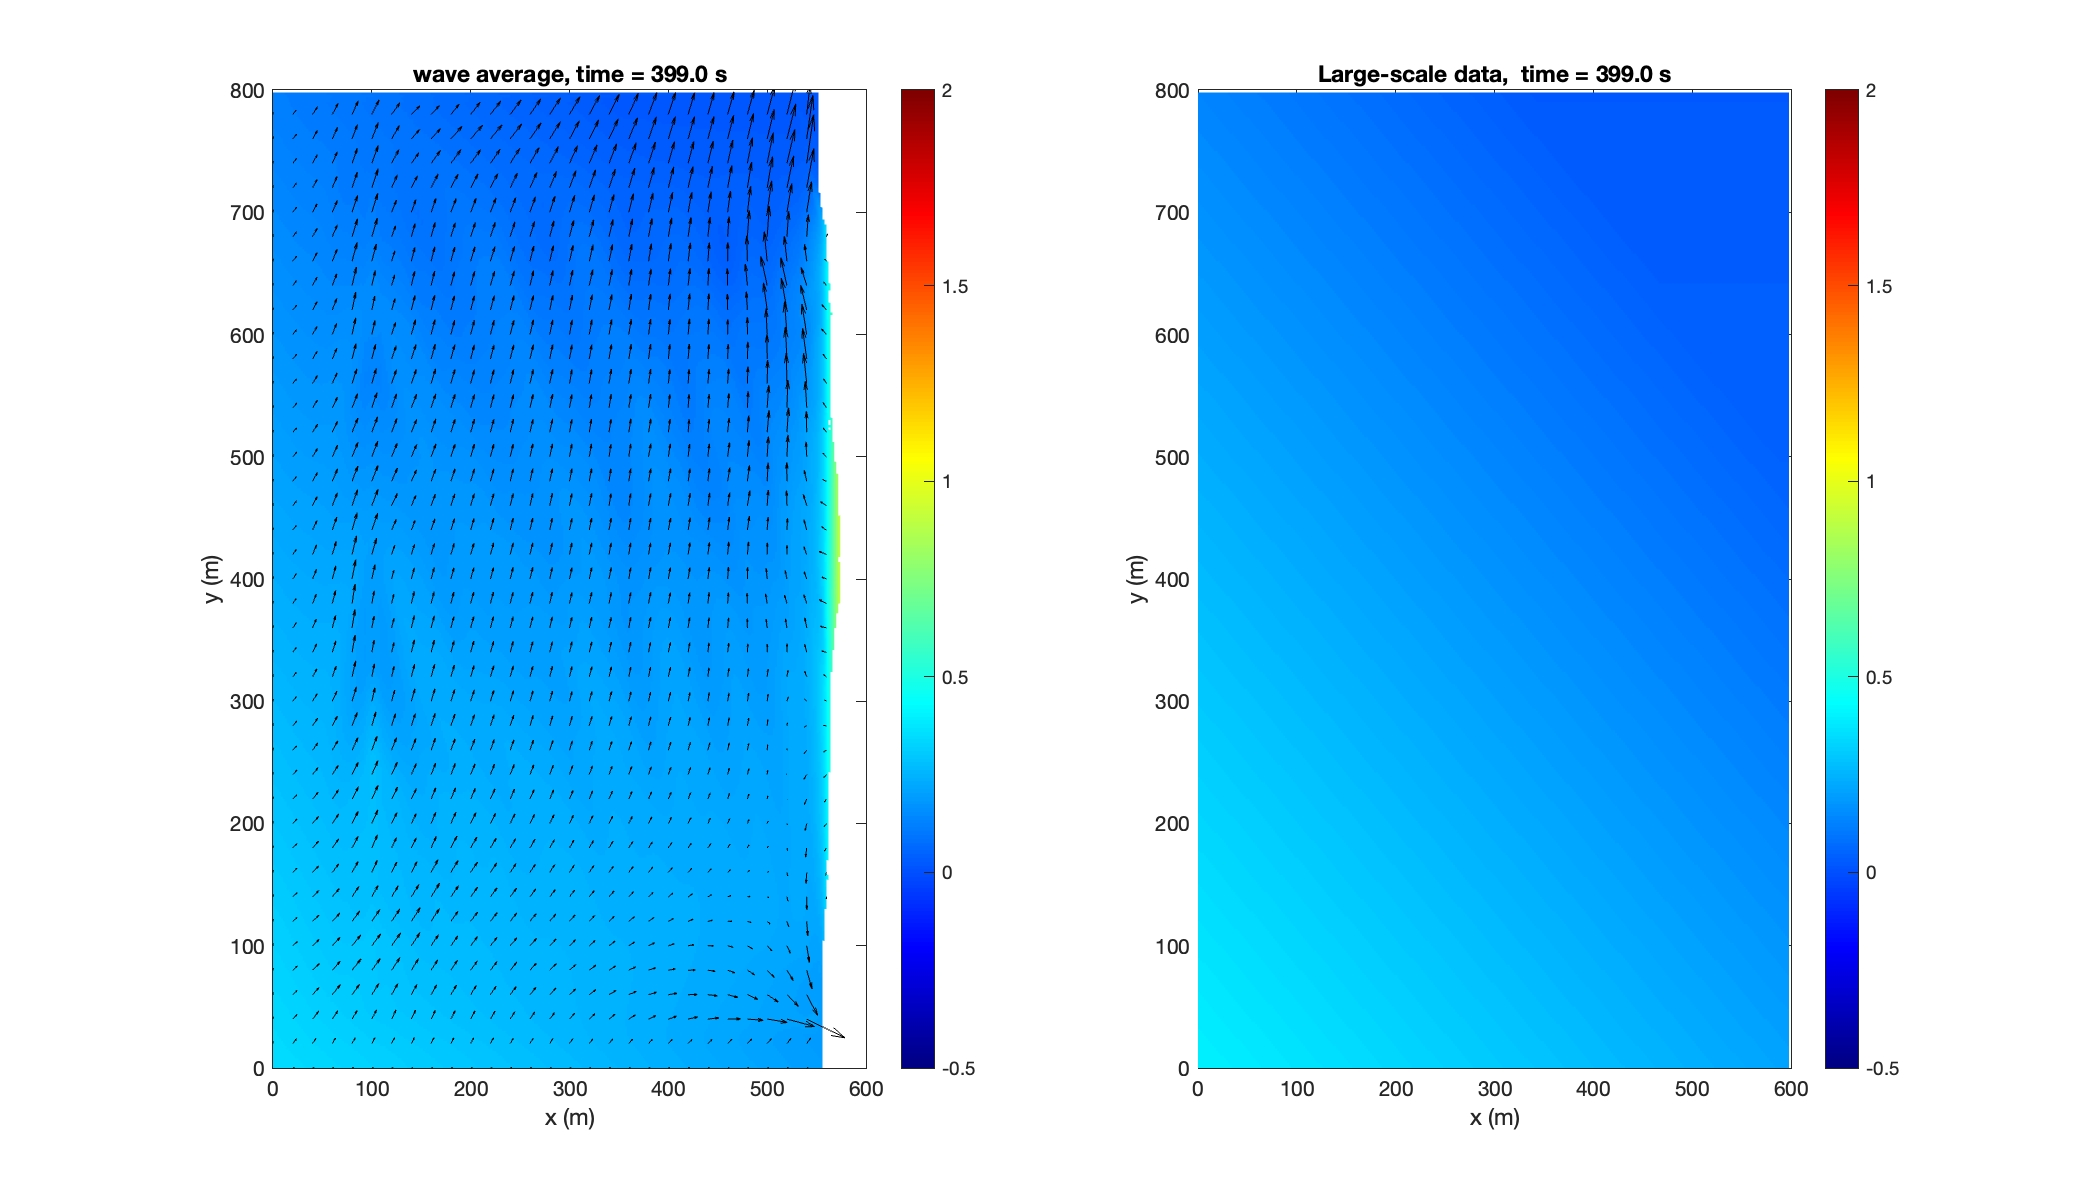
\includegraphics[width=1.0\textwidth]{figures/uvmean_view.jpg}
 \caption{Left: mean surface and mean velocity from FUNWAVE; right: surface elevation interpolated from the large-scale model }
 \label{mean}
 \end{center}
 \end{figure}  
  
  \section{Package}
  
  I updated the package in GITHUB. 
  
    \href{https://github.com/fengyanshi/TMA_MAKER}{https://github.com/fengyanshi/TMA\_MAKER}
  
  \section{TO DO}
  
  1) time-varying JON or TMA wavemaker?
  
  2) incorporate the time-varying spectra (the previous work) into this module. 
  
  3) something else.
  
\end{document}







